\section{Theory \& Background}
\subsection{The SIRS Model}

\label{section: SIRStheory}
The SIRS model is a compartmental model describing the distribution of agents existing in each compartment

\begin{itemize}
    \item Susceptible (S) - agents who are at risk of being infected by the disease,
    \item Infected (I) - agents who are infected by the disease and may pass on the disease to susceptible agents,
    \item Recovered (R) - agents who have recovered from the disease.
    
\end{itemize}

at a given time instance. It is a derivative of the simpler SIR model \cite{SIR}, including here the possibility of transitioning from the state of being 'removed' (recovered or deceased) into a state of being susceptible to future contagion. 
\begin{figure}[H]
    \centering
    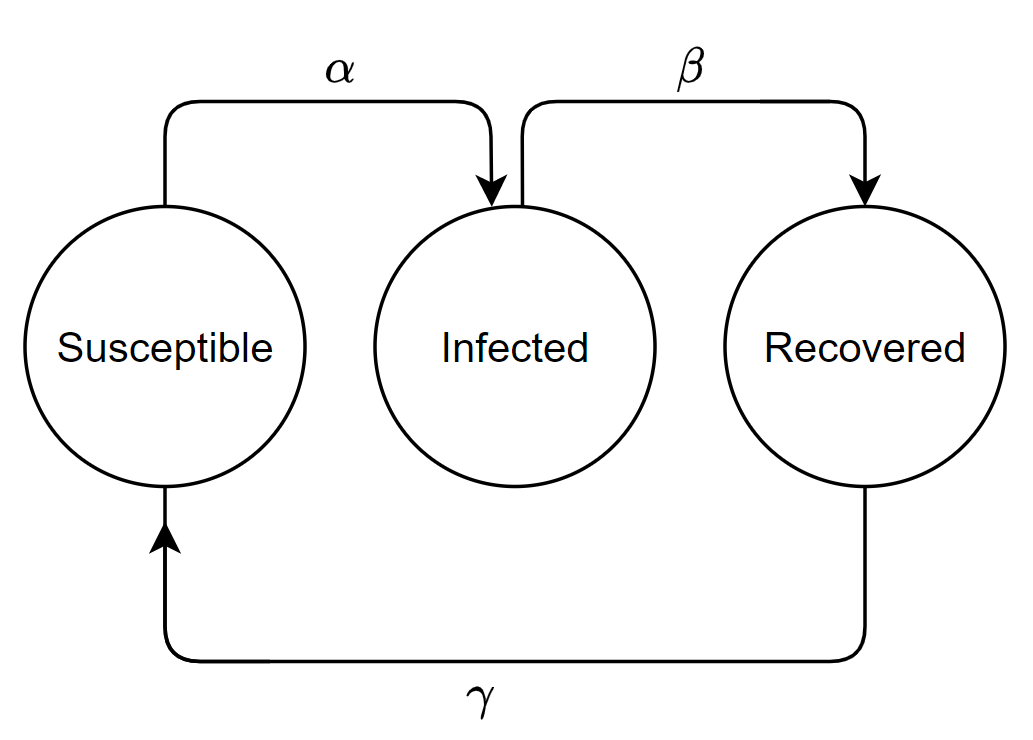
\includegraphics{Figures/SIR.PNG}
    \caption{A modular flow chart describing how agents move between the three compartments $S,\ I\ \text{and}\ R$.}
    \label{fig:SIRS}
\end{figure}
An agent may only transition between the network's compartments in a cyclic fashion as suggested by the model's name $S \overset{\alpha}{\to} I \overset{\beta}{\to} R \overset{\gamma}{\to} S$ with respective transition probabilities $\alpha, \ \beta\ \text{and} \ \gamma$. The transmission rate $\alpha$, recovery rate $\beta$ and immunity loss rate $\gamma$ all have units of inverse time. As an example, setting $\alpha = \beta = \gamma = 1$ / day implies that the agents in the network on average contacts, recovers from and loses immunity to the disease within one day and may be taken as a measure of how long the agent exists in a given compartment. In the deterministic picture, we view the occupation of each compartment as a temporally continuous variable such that the dynamics of compartmental transition is governed by the following set of ordinary \textit{non-linear}\footnote{This implicates sensitivity to initial conditions.} differential equations

\begin{align}
    \begin{split}
        S'(t) &= \gamma R(t) - \alpha S(t)I(t)/N\\
        I'(t) &= \alpha S(t)I(t)/N - \beta I(t)\\
        R'(t) &= \beta I(t) - \gamma R(t)
        \label{SIRS}
    \end{split}
\end{align}

where $N = S(t) + I(t) + R(t)$ is the total number of agents in the network, and is for our simplest simulations assumed to be constant as we here omit vital dynamics considerations such as birth rate and natural death rate, assuming then that disease evolves in the network on a time scale which is significantly shorter than the time scale spanning the average agent's lifetime. In the stochastic picture, however, we first observe that for a sufficiently small temporal step $\Delta t$, at most one agent moves from a given compartment to another. As 
$$
\begin{cases}
\text{max}\{\underbrace{\alpha SI\Delta t/N}_{S\to I}\} = \alpha N\Delta t/4\\

\text{max}\{\underbrace{\beta I\Delta t}_{I\to R}\} = \beta N\Delta t \\

\text{max}\{\underbrace{\gamma R \Delta t}_{R\to S}\} = \gamma N\Delta t
\end{cases}
$$
we may require that $\Delta t = \text{min}\{4/\alpha N, 1/\beta N, 1/\gamma N\}$ and reinterpret
$$
\begin{cases}
P(S\to I) = \alpha SI\Delta t/N\\\
P(I\to R) = \beta I\Delta t\\
P(R\to S) = \gamma R \Delta t
\end{cases}
$$

as transition probabilities. In this way, we may implement the SIRS model stochastically by generating (pseudo)random numbers and at each time step allow agents to move in and out of each compartment by proposing transitions and either accepting or rejecting them by measuring each transition probability against the random numbers. It should be duly noted that the SIRS model further works on the basis of the following assumptions\\

\begin{itemize}
    \item The population mixes homogeneously, id est every agent in the network is at all times equally likely to contact, recover and lose immunity to the disease.
    \item Following the homogeneity of the population, all the parameters describing transitions are averages.
    \item The disease has no pertaining incubation time. It is instantly transmitted, and those who contact the disease are immediately moved into compartment $I$.
    \item In the case of adding vital dynamics to the model, we assume that all newborns are initially susceptible.
\end{itemize}

\subsection{Improving the Model}\label{improvingmodel}
In this section we shall explore in what ways we may incorporate different realizations of the SIRS model in order to better capture the true nature of how infectious diseases may spread within a network. The layers of realism we add to the model in this project do not confer the possibility of making real - world predictions for the current, or any other, pandemic as this is a system with very complex behaviour in both temporal and spatial dimensions. Rather, it allows us to heuristically study their impact on the model.\\

In a first attempt of improving the model, we add the realization of vital dynamics across all compartments $S, \ I \ \text{and}\ R$. In many cases, the stages of  identification, outbreak and eradication of an infectious disease may all occur within a time span significantly shorter than the average lifetime of the agents within the network. However, in a few select cases, this is far from the truth. A few examples include the Ugandan trypanosomiasis epidemic (1900 - 1920)\cite{uganda}, the HIV/AIDS pandemic (1981 - present) and the Antonine Plague (165 - 180, Roman Empire)\cite{historypandemics}. Such long lasting diseases not only claim the lives of a significant percentage of the population, but their dynamics are also dependent on the in - and outflow of agents within the network. An improved modular scheme may be visualized as
\begin{figure}[H]
    \centering
    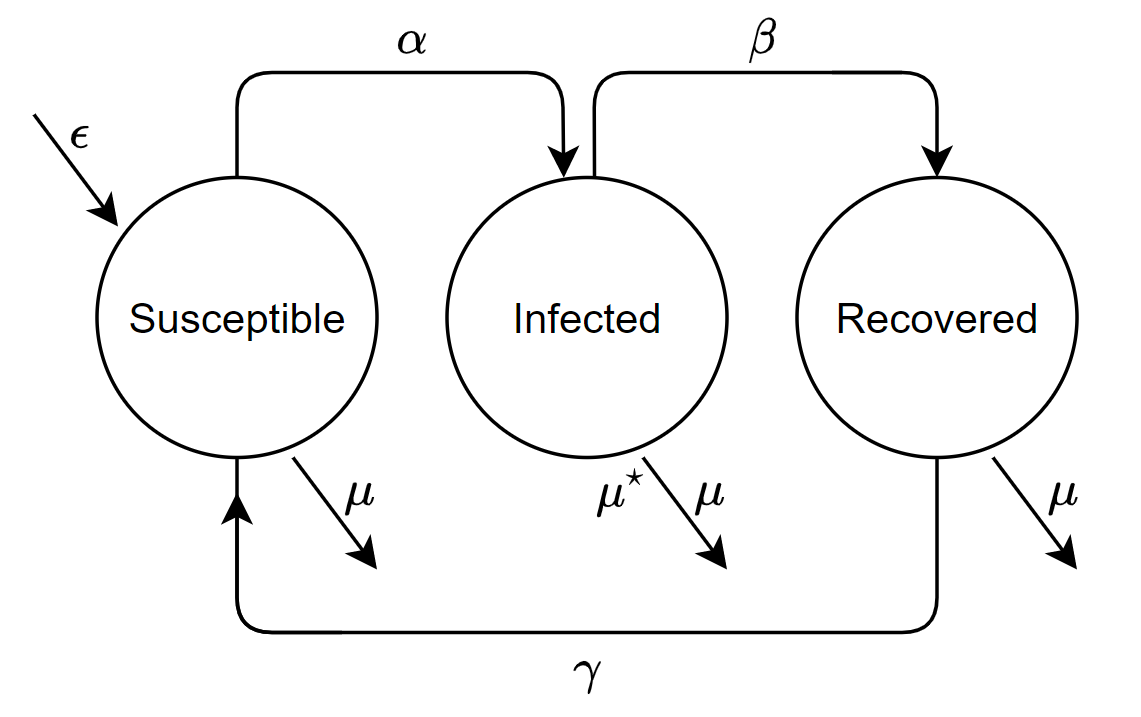
\includegraphics{Figures/SIRVITAL.PNG}
    \caption{A modular flow chart describing the motion of agents between the compartments $S, \ I\ \text{and}\ R$, now adding vital dynamics.}
    \label{SIRVITALCHART}
\end{figure}
where $\mu, \ \mu^\star \ \text{and} \ \epsilon$ denote the average death rate due to natural causes, the death rate due to the infectious disease and the average birth rate respectively. In the deterministic picture, we may construct a new set of differential equations
\begin{align}
    \begin{split}
        S'(t) &= \gamma R(t) - \alpha S(t)I(t)/N(t) - \mu S(t) + \epsilon N(t)\\
        I'(t) &= \alpha S(t)I(t)/N(t) - \beta I(t) - (\mu + \mu^\star)I(t)\\
        R'(t) &= \beta I(t) - \gamma R(t) - \mu R(t)
        \label{SIRS}
    \end{split}
\end{align}

where we now let the total number of agents in the network $N(t)$ be a continuous variable in time. For the stochastic simulation, we determine the temporal resolution $\Delta t$ in the same way as before, now adding the possible transitions $S\to D,\ I\to D \ \text{and} \ R \to D$ for a new compartment $D$ in which deceased agents are moved to, $I \to D_I$ for a new compartment $D_I$ in which agents who die from the disease are moved to, and $B \to S$ for a new compartment $B$ in which newborns are moved from. As before, we may then reconstruct new transition probabilities
$$
\begin{cases}
P(S\to D) = \mu S\Delta t\\
P(I\to D) = \mu I\Delta t\\
P(R\to D) = \mu R \Delta t\\
P(I\to D_I) = \mu^\star I \Delta t\\
P(B\to S) = \epsilon N \Delta t
\end{cases}
$$

As before, the vital dynamics realization will not allow us to make predictions of real - world statistical value, and now mainly because the provided examples of long lasting diseases are very complex in their transmission. HIV/AIDS is vertically transmitted, meaning that offspring are born with the disease, and the two other confer vector transmission, meaning that the disease is transmitted from animal carriers onto agents. Although we do not attempt to implement these conditions in this project, the additional layer of vital dynamics allow us to study the effect of death and birth in combination with the disease.\\

Many infectious diseases, after an initial outbreak, may after some time be categorized as an endemic disease. In this stage, the disease has strongly manifested at an non-zero equilibrium, around which the number of currently infected agents may fluctuate. Such fluctuations are largely conferred by seasonally variable transmission rates, and is the case for diseases like the 'flu' or measles. The variations themselves are to this day studied in detail as they are not fully understood, although the commonly accepted explanations are characteristic pathogen survival outside of host, and the behaviour of susceptible hosts\cite{seasonal1}\cite{seasonal2}. Pathogens like the rota - and noroviruses, causing the 'flu', survive in cold climates unlike many other pathogens, and therefore display annual peaks in infection rates during the colder months of the year. Similarly, measles are a common disease among children, and analysis shows that there is a strong correlation between the rate of infection and the conglomeration of children at school, after - school  activities and the alike, pertaining seasonal variation in transmission rates to the behavioural pattern of the pathogen's host. To model this realization in our program, we define the transmission rate as a function of time by 
\begin{equation}
    \alpha(t) = A\cos(\omega t) + \alpha_0
\end{equation}
in which $\alpha_0$ is the average transmission rate, $A$ is the amplitude of the variation, being the largest deviation from the average transmission rate, and $\omega$ denotes the frequency at which the transmission rate changes. A flow chart describing the dynamics now adding seasonal variation may be taken as Figure \ref{SIRVITALCHART}, substituting $\alpha$ for $\alpha(t)$.\\

In a last attempt to make our model more realistic, we study the effects of vaccination, too. Vaccination is a powerful tool, and in many cases absolutely necessary in order to eradicate a disease in a network. This works by breaking the cyclic nature of the SIRS model, as agents in the susceptible state may be vaccinated and move directly into the recovered state. Agents in the recovered state may be vaccinated such that their possibility of moving into the state of being susceptible becomes zero.
\begin{figure}[H]
    \centering
    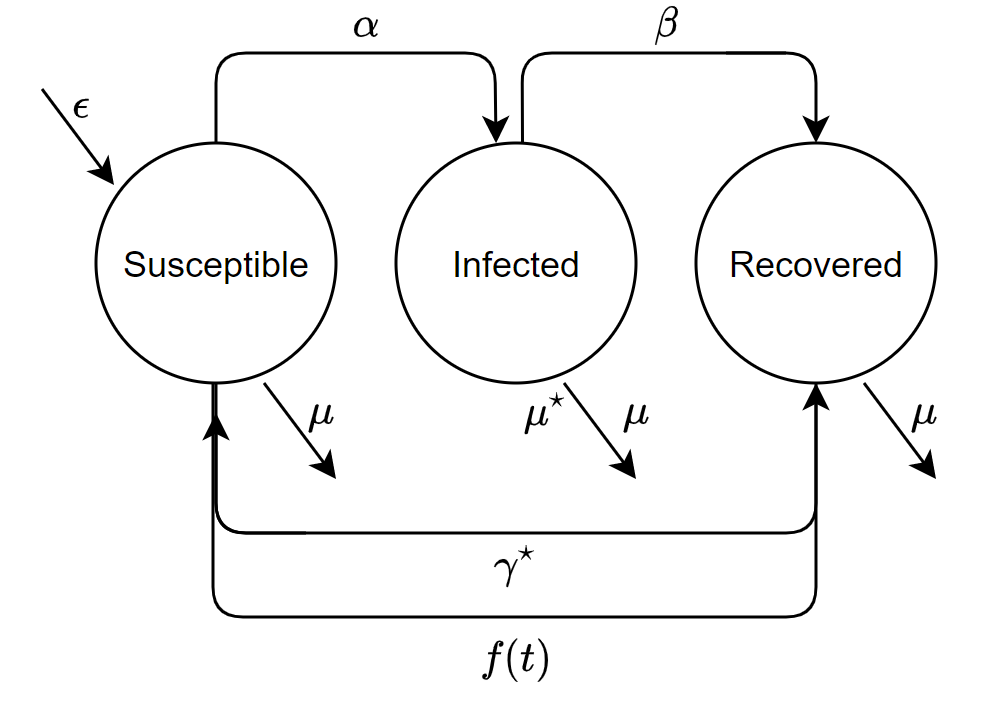
\includegraphics{Figures/sirvax.PNG}
    \caption{A final, compound modular flow chart describing all realizations of the SIRS model we have implemented.}
    \label{fig:sirsvax}
\end{figure}
Figure \ref{fig:sirsvax} describes the motion of agents in and out of the three different compartments, now having added the possibility of being vaccinated. This gives rise to $\gamma^\star$, still describing the rate of loss of immunity to the disease, but now only being applicable to agents occupying $R$ whilst not having been vaccinated.\\

For the deterministic approach, a new set of coupled differential equations emerges as

\begin{align}
    \begin{split}
        S'(t) &= \gamma R(t) - \alpha S(t)I(t)/N - f(t)\\
        I'(t) &= \alpha S(t)I(t)/N - \beta I(t)\\
        R'(t) &= \beta I(t) - \gamma R(t) + f(t)
        \label{SIRSvax}
    \end{split}
\end{align}
in which $f(t)$ describes how the rate of vaccination varies with time. It may also be taken as a constant rate. For the stochastic approach, the only change needed in our program is the added transition probability $P(S\to R) = f(t)\Delta t$. 

In this project we study two possible vaccination programs, one in which the agents in the network are continuously vaccinated by $f(t) = \exp(\delta t)$ for some constant $\delta$ as to realize the continuous development of vaccines and their exponentially growing availability. This is of course a highly idealized scenario as this is economically infeasible and rarely occurs. In the second attempt to realize a more common vaccination strategy, we add a rate of vaccination following
\begin{equation}
f(t) = 
    \begin{cases}
    \eta t, \ \ \text{if} \ \cos(t) > 0\\
    0, \ \ \text{else}
    \end{cases}
    \label{fig:pulsevac}
\end{equation}
where $\eta \in \mathbb{R}$. This implementation is meant to simulate pulse vaccination, in which select groups within a network (children, elderly) are vaccinated at regular intervals as a mean of eradicating a disease. As our implementation of the SIRS model does not differentiate between agents (homogeneous mixing), we may still choose to vaccinate a given percentage of the occupants of the Susceptible compartment. Although pulse vaccination programs, such as the Pulse Polio Programme in India are well established, the mathematical and numerical aspects are still in their infancy which is why we find it necessary to study the effects of such a realization, too. Even though the pulse functions devised in other numerical and/or mathematical research papers are more formalized than the one we have chosen to implement, equation \ref{fig:pulsevac} severs its purpose as a mathematical pulse, and is in addition very easy to reformulate\footnote{As an example, we studied regular non-increasing pulses, for which equation \ref{fig:pulsevac} returns a constant.}.\\
\newpage
\subsection{Initial Conditions, Equilibrium and Stability}
In this project we study four different networks

\begin{table}[H]
    \centering
    \begin{tabular}{l|l|l|l|l}
         & A & B & C & D\\
         \hline
         $\alpha$ & 4.0 & 4.0 & 4.0 & 4.0\\
         $\beta$ & 1.0 & 2.0 & 3.0 & 4.0\\
         $\gamma$ &0.5 &0.5 &0.5 &0.5\\
    \end{tabular}
    \caption{The transition rates for the four different networks we study.}
    \label{tab:initconditions}
\end{table}

In all four networks, each compartment is initialized as $S_0 = 300$, $I_0 = 100$ and $R_0 = 0$. Upon adding different layers of realistic improvements to our model, we have devised many different initial conditions, all of which will be specified in the presented results.\\

The set of equations \eqref{SIRS} define a conservative system as the population remains constant under the assumption that we may omit vital dynamics in the first place. By that, we eventually reach an equilibrium state $(S_\infty, I_\infty, R_\infty)$ for which it is possible to derive analytical values for the fraction of occupants in each compartment by setting each derivative equal to zero. We rather choose to give the total number of occupants in each compartment
at equilibrium by

\begin{align}
    \begin{split}
        S_\infty &= N\frac{\beta}{\alpha}\\
        I_\infty &= \frac{N(1-\frac{\beta}{\alpha})}{1+\beta\gamma}\\
        R_\infty &= \frac{N\beta}{\gamma}\frac{1-\frac{\beta}{\alpha}}{1+\frac{\beta}{\gamma}}
        \label{sirseq}
    \end{split}
\end{align}

Notice in \eqref{sirseq} that for any values of $\alpha$ and $\beta$ such that $\beta < \alpha$, the number of infected agents at equilibrium is non - zero. In this project we only study the effect of varying the rate of recovery $\beta$ in the simple SIRS model, mainly because this variable is more easily controllable by real - world health measures. It should be noted however, that the rate of transmission, or contact rate, is to some extent also controllable by imposing social measures such as wearing masks, increasing the availability of disinfectants or city-wide lockdown. We have not studied this parameter in detail as of now, as we rather would control this variable in a model which takes heterogeneous mixing into account, and is therefore a prospect for our future selves.   